\section{Coping with Cross Traffic}\label{s:queue-ctl}
\begin{figure*}[t]
    \centering
    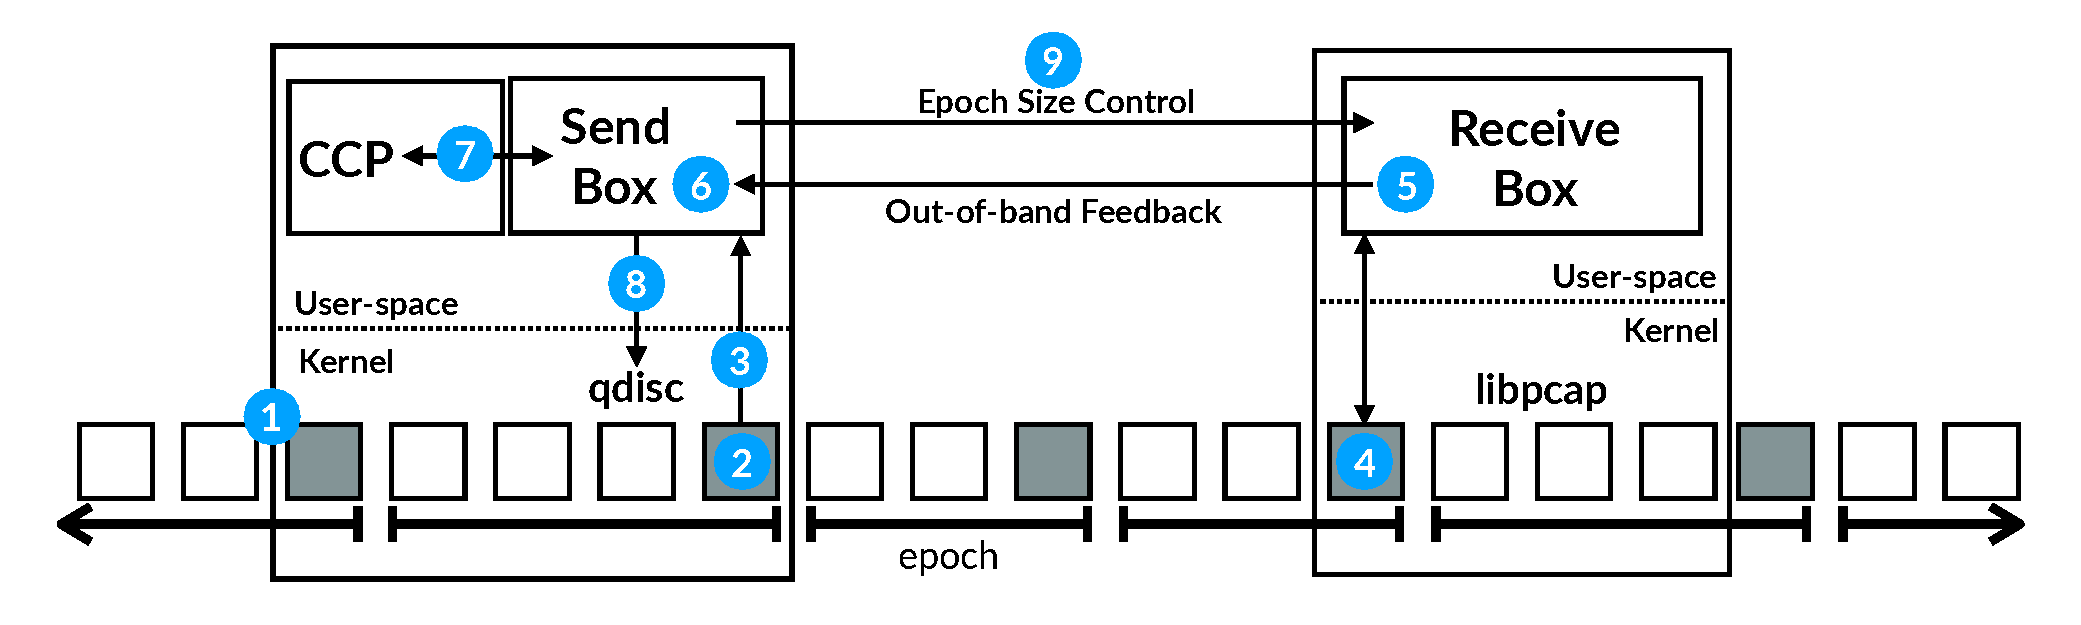
\includegraphics[width=2\columnwidth]{img/bundler-diagram}
    \vspace{-10pt}
    \caption{\name Implementation Overview. Box shading corresponds to the roles described in Figure~\ref{fig:design:block-diag}.}\label{fig:bundler}
\end{figure*}


Recall that \name's key trick is to use delay-minimizing congestion control algorithms from the bottleneck to the \inbox.
However, a well-known property of delay-minimizing congestion control algorithms is that when competing with traditional loss-based  controllers, they lose throughput~\cite{copa}.
Therefore, it is important for congestion controllers at the \inbox to detect the presence of such algorithms and disable the use of delay-control in these situations.
Once the buffer-filling cross traffic leaves, the \inbox should resume delay control.

\paragrapha{Competing Fairly}
What should the \inbox do when it detects the presence of buffer-filling cross traffic?
A naive approach would be to emulate the end-host behaviour and run Cubic. This approach has two shortcomings.
First, it must solve the MulTCP~\cite{multcp} problem: a bundle may comprise of multiple Cubic connections, and to achieve a fair bandwidth share it should therefore compete as aggressively as the number of component flows. 
On some high-performance datapaths, it may be difficult to measure this number~\cite{heavy-hitters}.

We propose a simpler solution.
Recall that bundles comprise of traditional end-host connections, with their own congestion controllers. 
If we simply \emph{let the traffic pass}, \ie increase the pacing rate at the \inbox to stop controlling queues as described in \S\ref{s:design:key}, these end-host congestion controllers will naturally compete fairly with cross traffic, just as traffic in the Internet does today.
\an{Copa is not compatible with this approach because its TCP-compatible mode is designed for the context of a single connection. Therefore, we must use Nimbus for cross traffic detection.}

\radhika{chop the above paragraph?}

\paragrapha{Active Probing}
When does the \inbox know it is safe to resume delay-control and scheduling?
Because bundles include buffer-filling cross traffic, it is important to distinguish between \emph{self-inflicted} queueing delay and queueing delay due to cross traffic.
When the queueing delay is purely self-inflicted, it is safe to resume control over the queues at the \inbox.
Passive probing is insufficient to determine this state, since passive measurements of the bottleneck will be identical in the case of self-inflicted queueing and queueing driven by cross traffic.
Therefore, it is important to \emph{actively probe}, that is, change the rate of in-band traffic and observe the response of the cross traffic. 
This is what the Nimbus mechanism does.
At a high level (see Appendix \S\ref{s:app:nimbus} for details),
Nimbus sinusoidally varies the sending rate $r(t) = A sin(\frac{4\pi{}t}{T})$ during the up-pulse, where $A$ is the pulse amplitude (set to one-fourth of the estimated bottleneck bandwidth) and $T$ is the pulse duration, and measures the cross traffic's response in the frequency domain.
The \inbox can use the Nimbus algorithm to detect when to relinquish control over the queue by interposing this sending pattern over the delay-controller's rate decisions.
However, this implies that we must be careful when letting the traffic pass; if the \inbox entirely drains its queues into the network, it will no longer be possible for Nimbus to overlay pulses onto the traffic pattern, and it will be unable to determine the nature of the cross traffic.
Practically, this would mean that once \inbox switches to compete with cross traffic, it would never gain the information necessary to switch back.

Instead, to support active probing while also letting the traffic pass, the \inbox must \emph{hold back} some packets.
How many packets should this be? The \inbox should be able to generate enough packets for a Nimbus up-pulse, \ie the area under the up-pulse curve: 
$A \int_0^{\frac{T}{4}} sin(\frac{4\pi{}t}{T}) dt = \frac{AT}{2\pi}$.
From Nimbus, we use $T = 0.2$ seconds and $A$ is as above, one-fourth the bottleneck bandwidth. By Little's law, we can calculate the amount of extra queueing: $\frac{T}{8\pi}$, or $8$ms.
We thus configure the \inbox to hold back $8$ms of queueing for active probing.
Note that this extra queueing is in addition to queueing in the network. As a result, the end-to-end Cubic connections will see RTT inflation, and experience slightly lower throughput due to RTT unfairness. 
In \S\ref{s:robust:cross} we show that this effect is not large; \name still achieves performance comparable to the status quo.

How should we achieve this target queueing delay? 
This problem is similar to the role of the PIE AQM mechanism~\cite{pie}, which also seeks to maintain a queueing delay target.
Correspondingly, we implement a PI controller at the \inbox as part of the fairness control module. 
It overlays a rate $r$ corresponding to $\dot{r}(t) = \alpha (q - q_T) + \beta (\dot{q})$, where $q$ is the queue size and $q_T$ is the target queue size computed above.
We pick $\alpha = 10$ and $\beta = 10$ as per \S\ref{s:qctl:pi}.

\begin{Appendix}
\section{Queue Controller Stability}\label{s:qctl:pi}

We control the queues with the update function 
    
    $\dot{r}(t) = \alpha (q - q_T) + \beta (\dot{q})$.

How should we set $\alpha$ and $\beta$? This decision is related to the size of the Nimbus pulse. 
If the queue controller is too aggressive (\ie it reacts quickly to maintain the queue target), it will nullify the Nimbus pulse with its overlaid rate control.
If it is too timid, it will not be able to effectively control the queues.

Therefore, we want the target queue length to be $A sin(\frac{2\pi{}t}{T})$. 
We can write how the queue length varies with time as 
    
    $\dot{q}(t) = \mu - r(t) - A sin(\frac{2\pi{}t}{T})$, where $\mu$ is the link bandwidth.

\noindent Thus, 
    
    $\ddot{q}(t) = - \dot{r}(t) - A \frac{2\pi{}t}{T} cos(\frac{2\pi{}t}{T})$.

\noindent Combining with the rate update rule:

$\ddot{q}(t) - \beta \dot{q}(t) + \alpha (q(t) - q_T) = A \frac{2\pi{}t}{T} cos(\frac{2\pi{}t}{T})$.

\noindent Substituting the pulse parameters from Nimbus and using $y(t) = q(t) - q_T$, we write a second-order ordinary differential equation (ODE) with sinusoidal input:

$\ddot{y}(t) - \beta \dot{y}(t) + \alpha y(t) = 10\pi{}A cos(10\pi{}t)$.

    \noindent This has the standard-form solution \an{todo cite a textbook}:

$y(t) = c_1 e^{r_1 t} + c_2 e^{r_2 t} + \frac{10\pi{}A}{|p(10\pi{}i|} cos(10\pi{}i - \phi)$ where $p$ is the characteristic polynomial and $r_1, r_2$ are its roots.

\noindent We want: (1) the $r_1$, $r_2$ to be large, so the queue converges quickly, and (2) the pulse amplitude to be approximately the Nimbus pulse amplitude, so:

$\frac{10\pi{}A}{|p(10\pi{}i|} = \frac{A}{5\pi}$.

$\alpha = 10, \beta = 10$ satisfy these constraints.
\end{Appendix}

% add plot varying queue length
% maybe measure the amount of time nimbus spent in the correct mode

% 3 iterations of the big experiment for comparison: reasonable qlen, too low, and too high

% 12: constant 48Mbps in the bundle and vary the cross traffic, don't vary within bundle, we expect it won't vary but we'll see
% 15: vary the amount of traffic in the bundle, larger range
% get both and then decide what to show 

% 14: broader number of bundles
